\documentclass{article}
\usepackage[paperwidth=2.7in,paperheight=4.1in,margin=0in]{geometry}
\usepackage{mathptmx}%{times}
\usepackage{graphicx}
\usepackage{siunitx}
\usepackage[absolute,overlay]{textpos}
\usepackage{color}

\setlength{\parindent}{0pt}
\begin{document}
\begin{textblock}{0.5}(2.8,5.3)
\normalsize
(a)
\end{textblock}
\begin{textblock}{0.5}(2.8,13.8)
\normalsize
(b)
\end{textblock}
\footnotesize
\hspace{0.06in}\input{../gravityWaves-btf/w-contour}

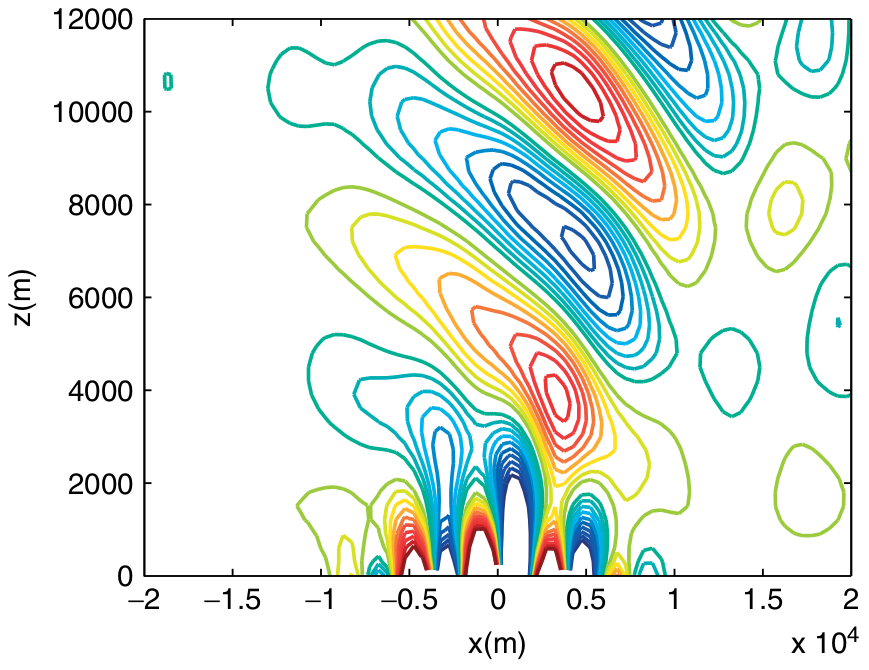
\includegraphics[height=2in]{img/melvin-7a.png}
\end{document}
